\chapter{Theoretical Model}
\label{theoretical-model}

In this chapter we will cover the structure of the codebook transfer model, as provided by Li \textit{et al.} \cite{10.5555/1661445.1661773}, and explore the variant proposed by Zang \textit{et al.}, called \textit{LKT-FM} \cite{10.1007/978-3-319-71246-8_39}.


\section{Codebook Transfer (CBT)}

CBT is a cross-domain recommender system aiming to transfer the rating pattern from a source domain to a target domain, to improve data quantity and provide better recommendations in the target domain. According to Li \textit{et al.} \cite{10.5555/1661445.1661773} CBT "can transfer useful knowledge from the auxiliary rating matrix in some other domains to remedy the sparsity of the rating matrix in a target domain".\\
Due to the nature of the model, we can distinguish three phases: codebook construction, codebook transfer and top-k recommendation.


\subsection{Input Data}

Input data provided to CBT model consists in two user-rating matrices. We call $URM_s$ the user-rating matrix of the source domain and $URM_t$ the user-rating matrix of the target domain.\\
While no user or item overlap is not required, CBT has only requirement for input data: the sparsity of the source dataset should be low enough to allow a meaningful amount of knowledge to be transferred. In \cite{10.5555/1661445.1661773} Li \textit{et al.} did not provide a functional sparsity percentage. In their experiment, the source dataset had a sparsity lower than 50\%.


\subsection{Codebook Construction}

Codebook construction exploits the assumption that, in CF, users with similar tastes or items with similar attributes behave similarly. For this reason, it is possible to compute user and item clusters to obtain a much more compact user-rating matrix of the source domain, which represents the groups behavior. The obtained compact user-rating matrix is called \textit{codebook}.\\
Li \textit{et al.} provided the following definition for \textit{codebook}:\\
"Codebook is a $k \times l$ matrix which compresses the cluster-level user-item rating patterns of $k$
user clusters and $l$ item clusters in the original rating matrix."\\
Once the codebook has been computed, an approximation of the original user-rating matrix can be retrieved.\par
\begin{figure}[hbt!]
  \centering
  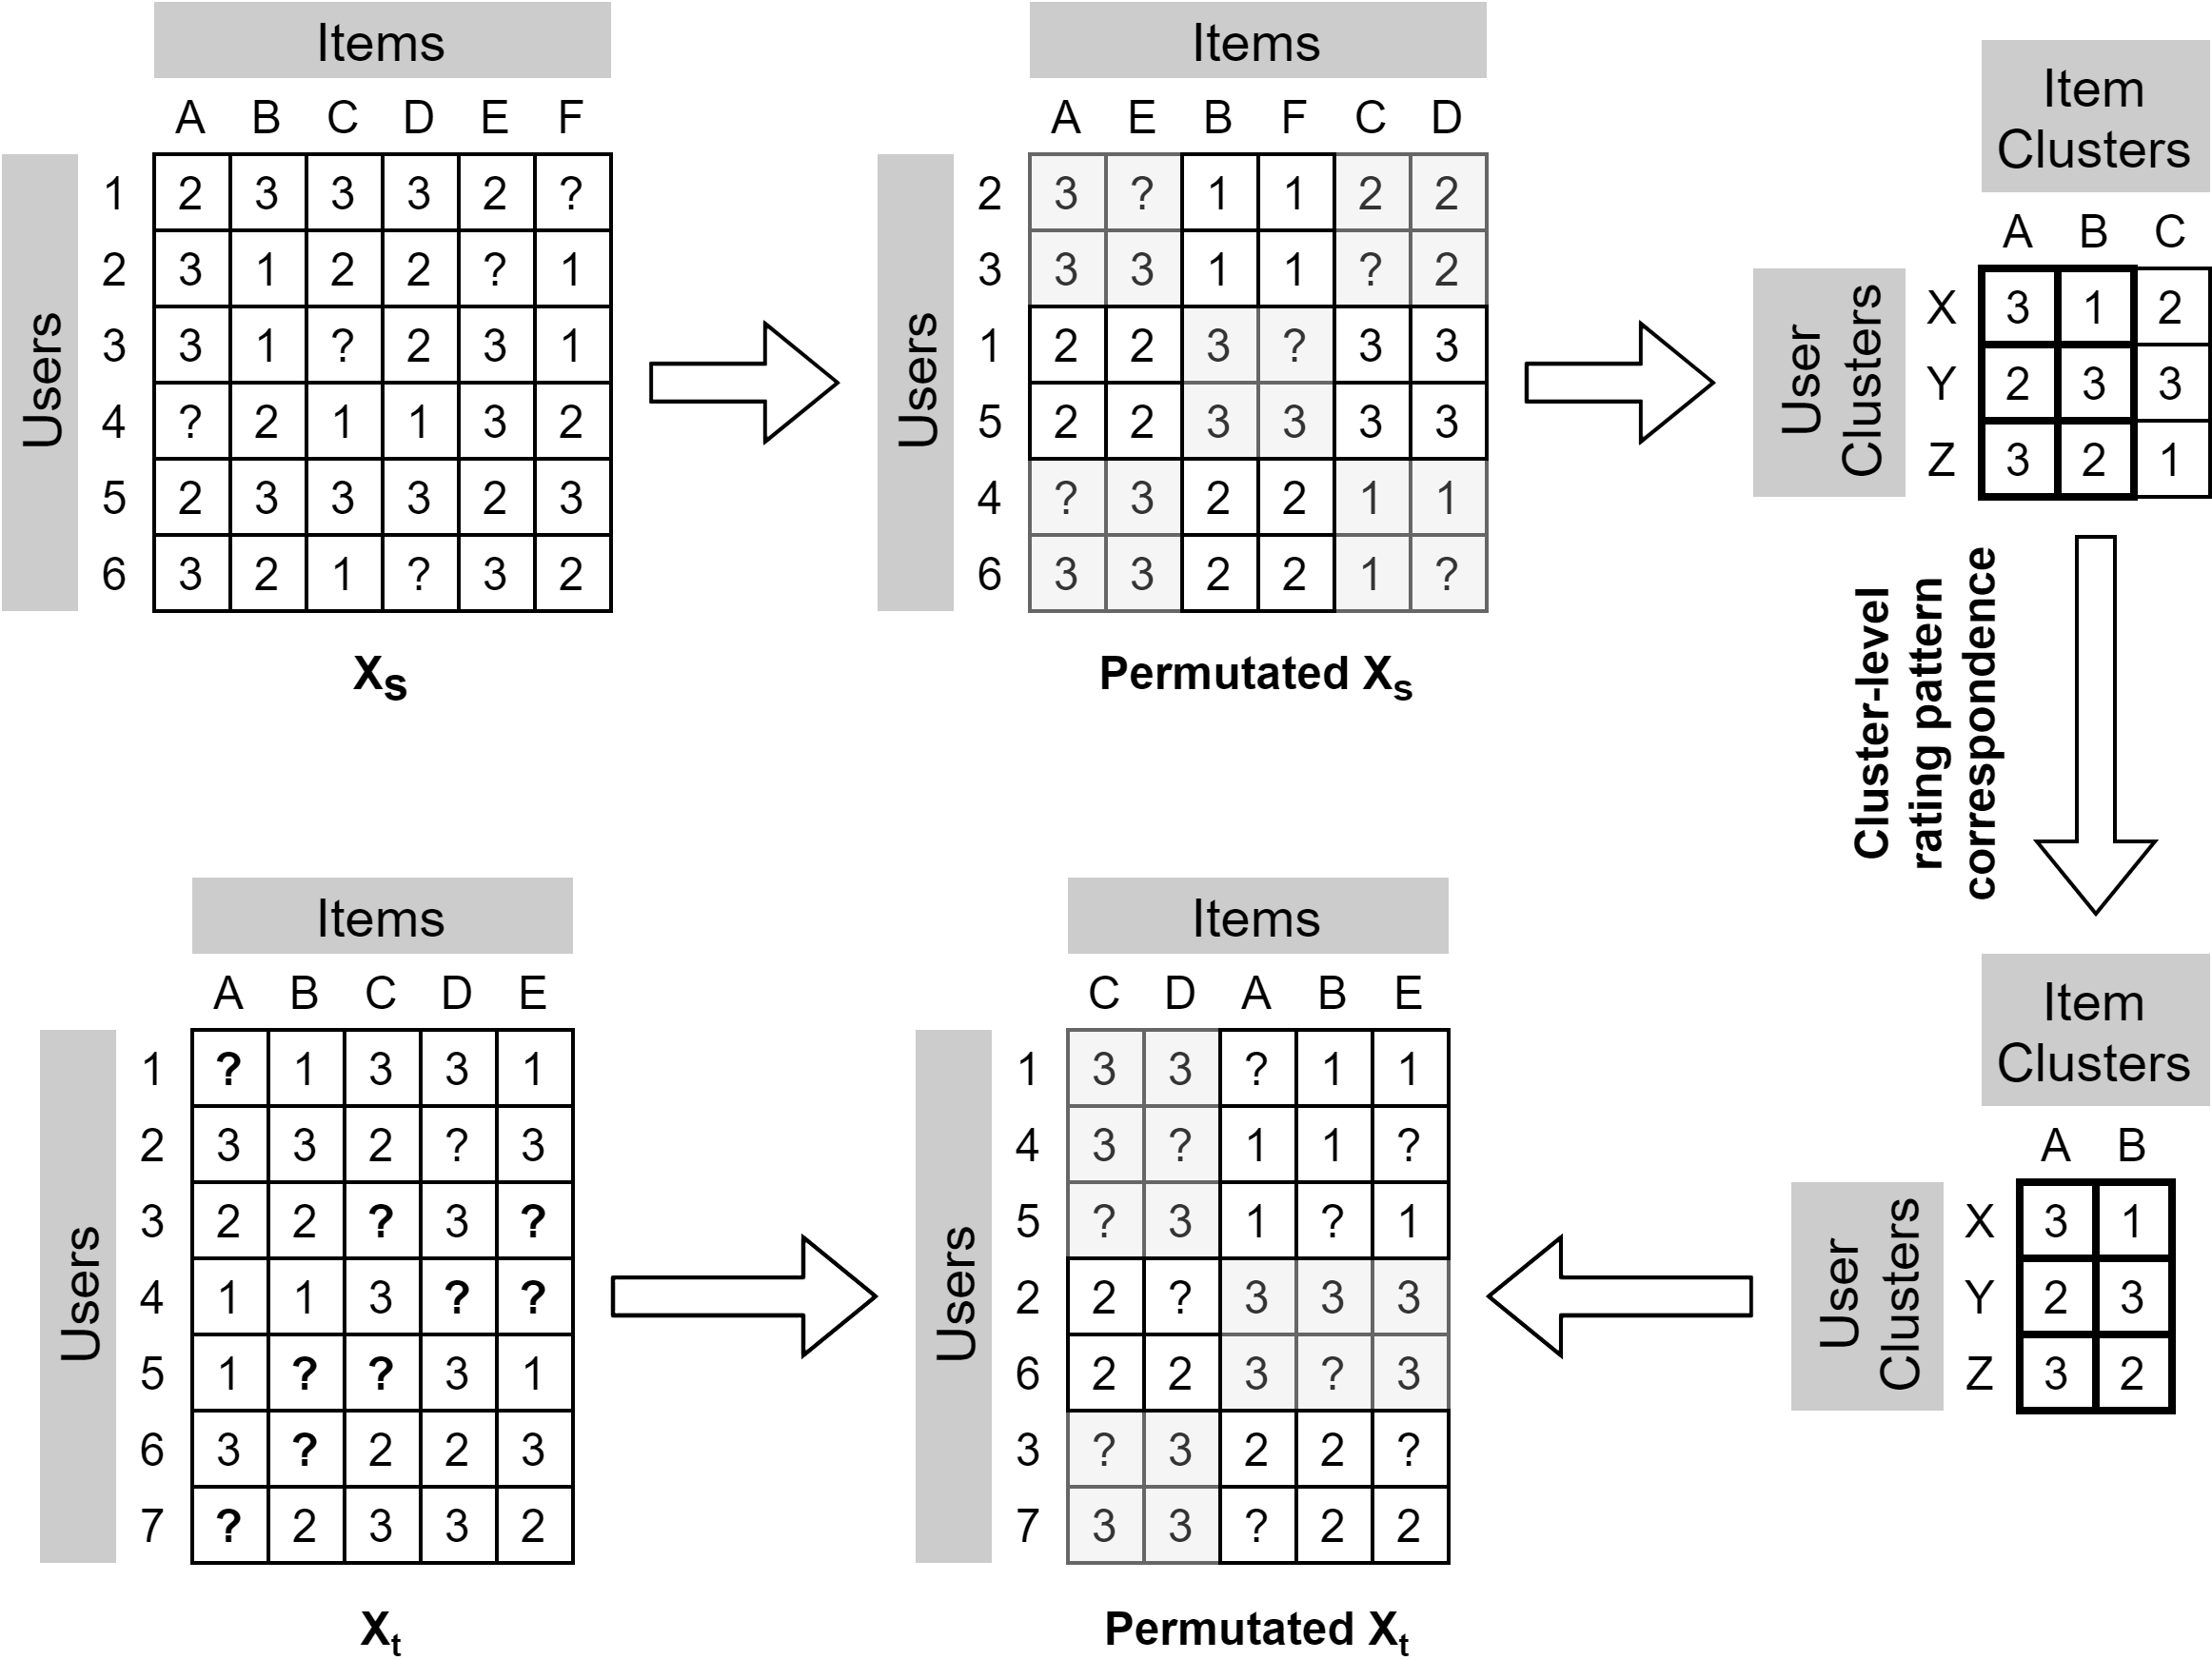
\includegraphics[width=0.8\textwidth]{pictures/codebook-construction}
  \caption{Example of codebook construction. Source: https://dl.acm.org/doi/10.5555/1661445.1661773}
\end{figure}
The codebook construction has to be performed by clustering users and items simultaneously. The authors adopted ONMTF \cite{10.1145/1150402.1150420} as the clustering algorithm. Thus, given a source user-rating matrix $X_s$ of shape $n \times m$ and a target codebook size $k \times l$, the optimization problem is the following:
\begin{equation}
\min_{U \in \mathbb{R}^{n \times k}_+, V \in \mathbb{R}^{m \times l}_+, S \in \mathbb{R}^{k \times l}_+} ||X_s - U S V^T||^2_F, \quad \text{s.t.} \quad U^TU = I, V^TV = I
\end{equation}
Where $U$ is the matrix of user clusters indicators and $V$ is the matrix of item clusters indicators.\\
Since it is sufficient to obtain a cluster hard membership indicator for each user and item, $U$ and $V$ are binarized to have only the non-negative entry in each row set to 1 and the others set to 0.\\
Once $U$ and $V$ are computed, the codebook $B$ is computed as follows:
\begin{equation}
B = \frac{U^T X_s V}{U^T 11^T V}
\end{equation}
The complete algorithm for codebook construction is the following:



\subsection{Codebook Transfer}


\subsection{Top-K Recommendations}



\section{LKT-FM}